\newpage
\section{Resultados e discussão}

% =============== EXPERIMENTO 1 ===================== %

\subsection{Determinação do Momento de Inércia de um disco}

Baseado no vídeo disponibilizado, logo abaixo temos uma tabela que reuni os valores medidos experimentalmente e que utilizaremos nos nossos cálculos para esse experimento:

\begin{table}[H]
    \centering
    \begin{tabular}{ |p{5cm}||p{2cm}||p{2cm}||p{2cm}|  }
        \hline
        \textbf{O que foi medido} & \textbf{Valor} & \textbf{Incerteza} & \textbf{Unidade}\\
        \hline
        Massa do anel (m\textsubscript{a}) & 0.9238 & \SI{\pm 0.0001} & kg\\
        Massa do disco (m\textsubscript{d}) & 0.4707 & \SI{\pm 0.0001} & kg\\
        Massa do eixo (m\textsubscript{e}) & 0.12125 & \SI{\pm 0.00001} & kg\\
        Comprimento do eixo (R) & 0.0060 & \SI{\pm 0.0001} & m\\
        Raio menor do disco (R\textsubscript{d1}) & 0.0060 & \SI{\pm 0.0001} & m\\
        Raio maior do disco (R\textsubscript{d}) & 0.0625 & \SI{\pm 0.0001} & m\\
        Raio menor do anel (R\textsubscript{a1}) & 0.0625 & \SI{\pm 0.0001} & m\\
        Raio maior do anel (R\textsubscript{a}) & 0.0660 & \SI{\pm 0.0001} & m\\
        \hline
    \end{tabular}
    \caption{Dimensões do Disco de Maxwell}
\end{table}

\begin{table}[H]
    \centering
    \begin{tabular}{ |p{5cm}||p{2cm}||p{2cm}||p{2cm}|  }
        \hline
        \textbf{O que foi medido} & \textbf{Valor} & \textbf{Incerteza} & \textbf{Unidade}\\
        \hline
        Altura (h) & 0.467 & \SI{\pm 0.001} & m\\
        Tempo de queda 1 (t\textsubscript{b1}) & 0.312 & \SI{\pm 0.001} & s\\
        Tempo de queda 2 (t\textsubscript{b2}) & 0.311 & \SI{\pm 0.001} & s\\
        Tempo de queda 3 (t\textsubscript{b3}) & 0.312 & \SI{\pm 0.001} & s\\
        \hline
    \end{tabular}
    \caption{Dados experimentais do Disco de Maxwell}
\end{table}

- momento de inércia das partes + incerteza\\
- momento para cada lanceamento (3x) + incerteza => determinar a media?\\
- compare os resultados

% =============== EXPERIMENTO 2 ===================== %

\subsection{Choques Rotacionais}

aaaaaaaaaa



% =============== EXPERIMENTO 3 ===================== %

\subsection{Conservação do Momento Angular}

Os conceitos da física estão presente em basicamente todas as nossas ações, e muitas vezes, não fazemos relação da teoria com a prática. Um caso muito elementar, mas muito interessante de ser analisado, são os movimentos de atletas de diferentes modalidades, os quais utilizam um mesmo conceito físico:  conservação do Momento Angular.

A Lei de Conservação da Quantidade de Movimento (ou Momentum) Angular diz que “se o torque externo resultante sobre um sistema em relação a um ponto é zero, então a quantidade de movimento angular total do sistema em relação ao mesmo ponto permanece constante”. Dessa forma: 

\[L = I  \omega\]

\[T_{ext sist} = \frac{\partial L_{sis}}{\partial t} = 0 \xrightarrow{} L_{sis} = cte\]

Na conservação de L: 

\[I_1 \omega _1 = I_2 \omega _2 \]

Então se I aumenta, $\omega$ diminui, para compensar e manter constante o momento angular do sistema.\\
 
\textbf{a) Baseado nos links fornecidos na vídeo-aula, escreva uma resenha sobre como muitos dos saltos acrobáticos realizados por atletas de alto desempenho podem ser entendidos utilizando a conservação do momentum angular.}\\

Com base em uma série de exemplos – incluindo aqueles apresentados nas vídeo-aulas dos experimentos – escolhemos algumas situações para exaltar o uso de tais conceitos no âmbito esportivo. Os casos mais comuns são os saltos ornamentais, a patinação no gelo, e a ginastica artística, seja nos movimentos de solo ou nas barras.\\

Usaremos esses exemplos para demonstrar como a conservação do momentum angular propicia tais feitos. Inicialmente, podemos falar do salto de trampolim. Sabemos que o centro de massa descreve uma trajetória parabólica e o atleta deixa o trampolim com um momento angular L em relação a um eixo horizontal que passa pelo centro de massa. Quando a mergulhadora está no ar, não fica sujeita a nenhum torque externo e, assim, o momento angular não varia. Quando a atleta fecha os braços e as pernas – levando-os para perto do corpo e consequentemente do centro de massa -, diminui o momento de inércia em torno desse eixo e assim, aumenta sua velocidade angular.\\

Quando a atleta abre as pernas e braços (passa da posição “carpada” para a posição esticada) no fim do movimento, o momento de inércia aumenta e sua velocidade angular diminui (mantendo a proporcionalidade do momento angular), permitindo que a atleta mergulhe quase sem espirrar água. Tal movimento só é possível graças à ausência de torque externo, que permite que o momento angular se conserve. \\

\begin{figure}[H]
  \centering
  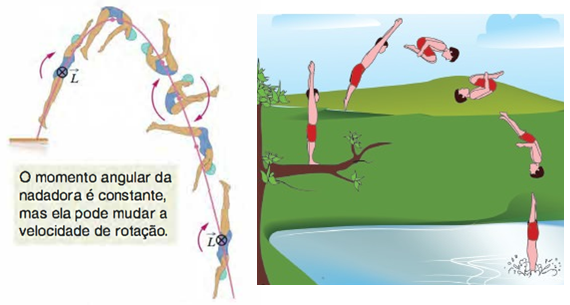
\includegraphics[scale=1.3]{images/i1.png}
  \caption{Saltos Ornamentais}
\end{figure}

O mesmo ocorre para os atletas da patinação no gelo. Como o torque exercido pelo piso de gelo no patinador é muito baixo – quase irrisório -, podemos considerar o momento angular praticamente constante, pois tratamos o sistema gelo + patinador como um sistema isolado. Dessa forma, quando ele recolhe os braços e pernas (aproximando-os do corpo), diminui consideravelmente seu momento de inércia, fazendo com que sua velocidade angular aumente e ele passa a girar com maior rapidez.\\ 

\begin{figure}[H]
  \centering
  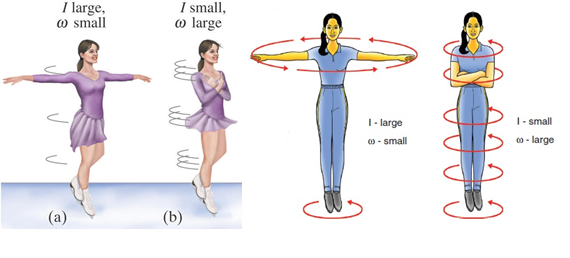
\includegraphics[scale=1.3]{images/i2.png}
  \caption{Patinação no Gelo}
\end{figure}

Analogamente, os ginastas das barras fixas utilizam a conservação do momento angular para realizarem seus movimentos de giro, ganhando ou perdendo velocidade conforme abrem ou fecham os braços e as pernas. \\

\begin{figure}[H]
  \centering
  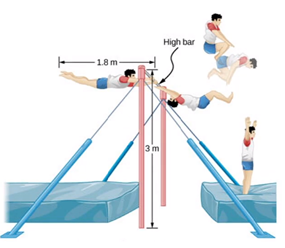
\includegraphics[scale=1.7]{images/i3.png}
  \caption{Ginástica - Barra Fixa }
\end{figure}

Então, mostramos a importância da lei de conservação do momento angular, que aplicada em sistemas isolados (ou quase isolados) nos fornece saltos e movimentos majestosos. Porém, em alguns casos essa conservação é motivo de alerta para nós.\\

Um exemplo desse, muito comum em veículos de manobras que realizam saltos, como motos e carros \textit{off-road}, pode ser observado nas competições de Mini Baja. Quando o carro salta de uma rampa e está no ar, não há torques externos agindo nele, então consideramos seu momento angular praticamente constante. Dessa maneira, a rotação das rodas é a responsável pela velocidade angular desse sistema, portanto, se frearmos diminuímos essa velocidade, e o carro como um todo tende a rotacionar no mesmo sentido das rodas (para frente), para compensar a falta de giro das rodas – por conta da conservação de momento-, fazendo com que o carro capote se frearmos com ele no ar. 
Caso realizemos o contrário, acelerando o carro com ele no ar, o chassi como um todo irá rodar no sentido oposto do aumento de velocidade das rodas (para trás) para compensar essa velocidade angular “positiva” nas rodas, mantendo constante o momento angular do sistema.\\ 

\textbf{b) Explique a demonstração do momento de inércia variável (banquinho giratório) apresentado na vídeo-aula.}\\

Ao estudarmos o assunto da conservação do momento angular, alguns exemplos clássicos são apresentados aos alunos. Um dos mais famosos, que tem fácil execução e pode ser feito até em sala de aula, é o experimento do “Banquinho Giratório”. Nesse exemplo, um banco – com pouco ou quase nenhum atrito – gira livremente em torno de um eixo vertical. Com a ajuda de rolamentos, que minimizam a força de atrito, podemos considerar o sistema banco + aluno como um sistema isolado, sem torques externos.\\

O estudante senta no banco e é posto em rotação com uma pequena velocidade angular inicial $\omega _1$, segurando dois halteres com os braços abertos. O vetor momento angular inicial L do aluno aponta para cima e está no mesmo eixo da rotação do banco. O estudante leva os halteres para próximo do peito, diminuindo o momento de inércia do valor inicial I$_1$ para um valor menor I$_2$ pois a massa dos halteres se aproxima do eixo de rotação. A velocidade angular do estudante aumenta consideravelmente, de $\omega _1$ para $\omega _2$, para poder compensar a diminuição do momento de inércia, conservando o momento angular. O estudante pode reduzir sua velocidade angular abrindo os braços novamente, afastando os halteres do eixo de rotação. Como já ressaltado, nenhum torque externo resultante age sobre o sistema formado pelo estudante, o banco e os halteres. Assim, o momento angular do sistema em relação ao eixo de rotação permanece constante, não importando como o estudante segura os halteres.

\begin{figure}[H]
  \centering
  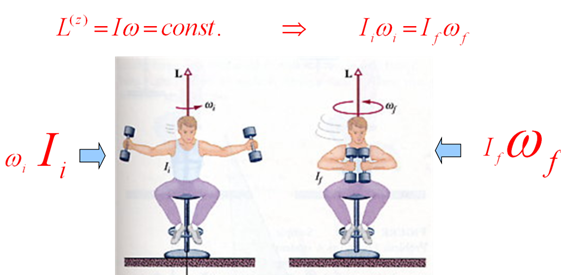
\includegraphics[scale=1.3]{images/i4.png}
  \caption{Banco Giratório}
\end{figure}

\textbf{c) Na vídeo-aula é apresentado a famosa demonstração do banquinho giratório com a roda de bicicleta. Explique o que acontece. Nas duas situações apresentadas como A e B indique o sentido de rotação da roda de bicicleta, justificando a sua resposta.}\\

Ainda podemos ressaltar um último experimento muito interessante que é o caso do banquinho giratório com a roda de bicicleta. Semelhantemente ao experimento anterior, um aluno senta em um banco, que gira sem atrito - não existindo torques externos sobre o sistema estudante-banco-roda, sendo considerado isolado. O aluno segura uma roda de bicicleta e no começo do experimento tanto o banco quanto a roda estão em repouso.\\

Em um certo momento a roda de bicicleta – que se encontra na horizontal – é posta para girar, criando um momento angular de rotação da roda, vertical. Quando o aluno levanta a roda, cria-se uma componente do momento angular ao longo do eixo z (para cima). Como o sistema é isolado, o momento angular deve ser conservado, então o banco começa a girar no sentido oposto da rotação da roda, de modo a criar um momento angular contrário ao criado pela roda.\\

Nesse experimento fica clara a conservação de momento angular na direção z (eixo para cima), pois inicialmente não havia momento nesse eixo. Ao inclinar a roda, surge uma componente de momento nesse eixo, no mesmo sentido da rotação imposta à roda de bicicleta. Mais que depressa, o banquinho começa a rodar no sentido oposto, para compensar a rotação que surge, buscando conservar o momento naquele eixo (que era nulo no início). No experimento do vídeo, não sabemos qual o sentido inicial de rotação da roda de bicicleta (que está coberta por um tampão), e são dadas duas situações:

\begin{itemize}
    \item Ao levantar a roda, o banco gira no sentido HORÁRIO.
    \item Ao levantar a roda, o banco gira no sentido ANTI-HORÁRIO.
\end{itemize}

Desse modo, como já discutimos acima, quando surge a componente do momento no eixo z, o banco gira no sentido oposto da roda para compensar essa rotação, então:

\begin{figure}[H]
  \centering
  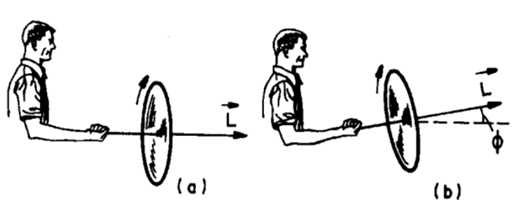
\includegraphics[scale=1.4]{images/i5.png}
  \caption{Roda de Bicicleta Giratória}
\end{figure}

\begin{figure}[H]
  \centering
  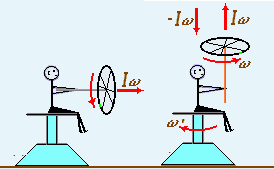
\includegraphics[scale=1.7]{images/i6.png}
  \caption{Banco Giratório com Roda de Bicicleta}
\end{figure}

\begin{itemize}
    \item Como o banco gira no sentido HORÁRIO, a roda inicialmente foi posta para girar no sentido ANTI-HORÁRIO.
    \item Como o banco gira no sentido ANTI-HORÁRIO, a roda inicialmente foi posta para girar no sentido HORÁRIO.
\end{itemize}



% =============== EXPERIMENTO 4 ===================== %

\subsection{Precessão do Giroscópio}

Baseado no video disponibilizado para esse experimento os dados que temos disponíveis são os seguintes:

\begin{table}[H]
    \centering
    \begin{tabular}{ |p{5cm}||p{2cm}||p{2cm}||p{2cm}|  }
        \hline
        \textbf{O que foi medido} & \textbf{Valor} & \textbf{Incerteza} & \textbf{Unidade}\\
        \hline
        Meio eixo (D) & 0.0565 & \SI{\pm 0.0001} & m\\
        Diâmetro do eixo (d\textsubscript{eixo}) & 0.0070 & \SI{\pm 0.0001} & m\\
        Raio externo (R\textsubscript{1}) & 0.0702 & \SI{\pm 0.0001} & m\\
        Raio interno (R\textsubscript{2}) & 0.0625 & \SI{\pm 0.0001} & m\\
        Largura externa (l\textsubscript{1}) & 0.0203 & \SI{\pm 0.0001} & m\\
        Largura interna (l\textsubscript{2}) & 0.0043 & \SI{\pm 0.0001} & m\\
        Massa do conjunto (M) & 1.116 & \SI{\pm 0.001} & kg\\
        Densidade do material ($\rho _{aco}$) & 8000.0 & - & $\frac{kg}{m^3}$\\
        \hline
    \end{tabular}
    \caption{Dados físicos do Giroscópio}
\end{table}

\begin{table}[H]
    \centering
    \begin{tabular}{ |p{5cm}||p{2cm}||p{2cm}||p{2cm}|  }
        \hline
        \textbf{O que foi medido} & \textbf{Valor} & \textbf{Incerteza} & \textbf{Unidade}\\
        \hline
        Tempo 1-1 (t\textsubscript{11}) & 0.072 & \SI{\pm 0.001} & s\\
        Tempo 1-2 (t\textsubscript{12}) & 0.135 & \SI{\pm 0.001} & s\\
        Tempo 1-3 (t\textsubscript{13}) & 0.194 & \SI{\pm 0.001} & s\\
        Velocidade 1 ($\omega _1$) & 271.2 & \SI{\pm 0.1} & $\frac{rad}{s}$\\
        \hline
        Tempo 2-1 (t\textsubscript{21}) & 0.073 & \SI{\pm 0.001} & s\\
        Tempo 2-2 (t\textsubscript{22}) & 0.138 & \SI{\pm 0.001} & s\\
        Tempo 2-3 (t\textsubscript{23}) & 0.198 & \SI{\pm 0.001} & s\\
        Velocidade 2 ($\omega _2$) & 255.6 & \SI{\pm 0.1} & $\frac{rad}{s}$\\
        \hline
        Tempo 3-1 (t\textsubscript{31}) & 0.076 & \SI{\pm 0.001} & s\\
        Tempo 3-2 (t\textsubscript{32}) & 0.144 & \SI{\pm 0.001} & s\\
        Tempo 3-3 (t\textsubscript{33}) & 0.206 & \SI{\pm 0.001} & s\\
        Velocidade 3 ($\omega _3$) & 308.2 & \SI{\pm 0.1} & $\frac{rad}{s}$\\
        \hline
        Tempo 4-1 (t\textsubscript{41}) & 0.074 & \SI{\pm 0.001} & s\\
        Tempo 4-2 (t\textsubscript{42}) & 0.142 & \SI{\pm 0.001} & s\\
        Tempo 4-3 (t\textsubscript{43}) & 0.205 & \SI{\pm 0.001} & s\\
        Velocidade 4 ($\omega _4$) & 256.4 & \SI{\pm 0.1} & $\frac{rad}{s}$\\
        \hline
    \end{tabular}
    \caption{Dados experimentais do Giroscópio}
\end{table}

- Estimar a massa do giroscópio\\
- Calcular o momento de inercia dele\\
- Frequência estimada (4x) \\
\\
- Frequência real (4x)\\
- Determinar diretamente (pelo tempo) a frequência de precessão\\
- Comparar as frequências
